\comment{Suggestion: past tense}\\

\subsection{Gradient Descent analysis}
    \begin{figure*}
        \begin{subfigure}{.5\textwidth}
            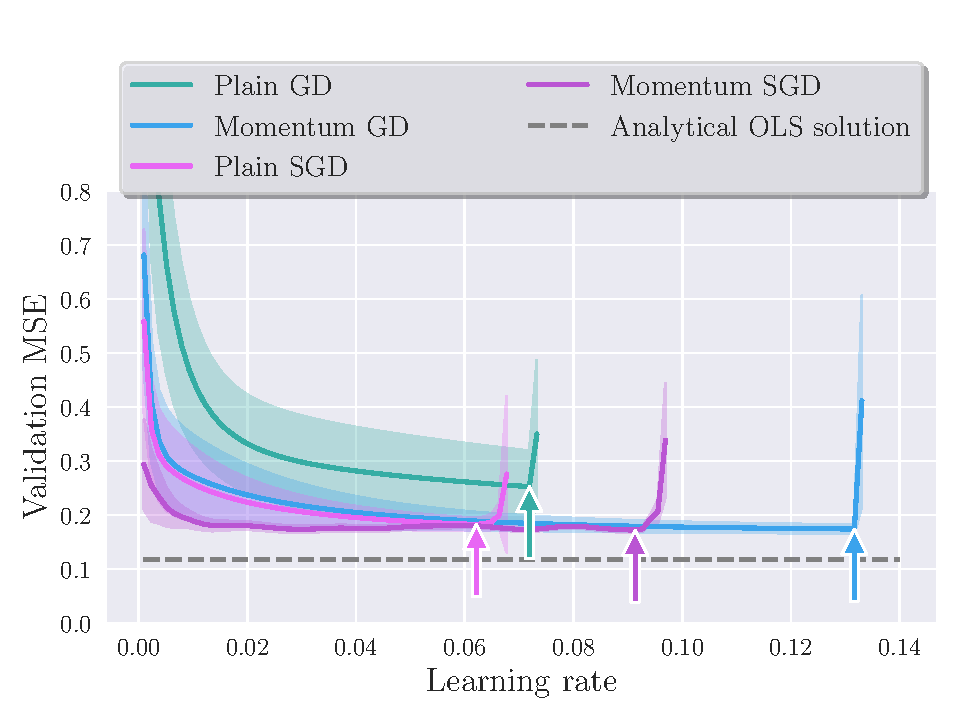
\includegraphics[width=\linewidth]{learning_rates_PGD_MGD_PSGD_MSGD.pdf}
            \caption{Best MSEs, learning rates: (0.2522, 0.0719), (0.1738, 0.132), (0.1787, 0.0399), (0.1755, 0.00934)}
            \label[fig]{res:fig:lrate1}
        \end{subfigure}
        \hfill
        \begin{subfigure}{.5\textwidth}
            \centering
            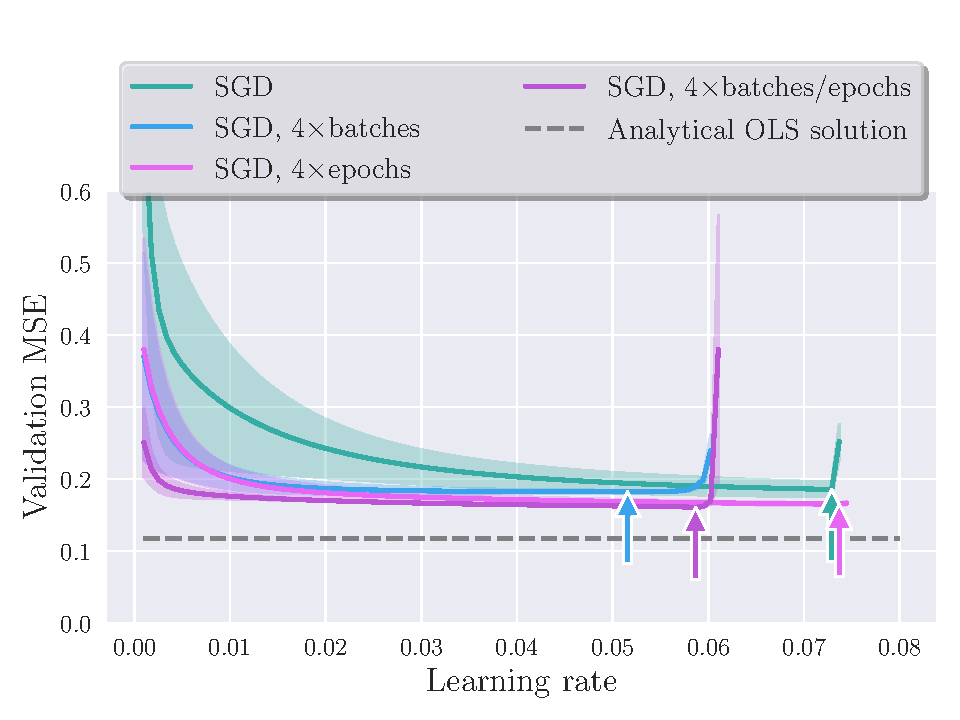
\includegraphics[width=\linewidth]{learning_rates_SGD_batches_epochs.pdf}
            \caption{Best MSEs, learning rates: (0.1787, 0.0402), (0.1746, 0.0152), (0.1703, 0.0343), (0.1697, 0.00394)}
            \label[fig]{res:fig:lrate2}
        \end{subfigure}
        \hfill
        \begin{subfigure}{.5\textwidth}
            \centering
            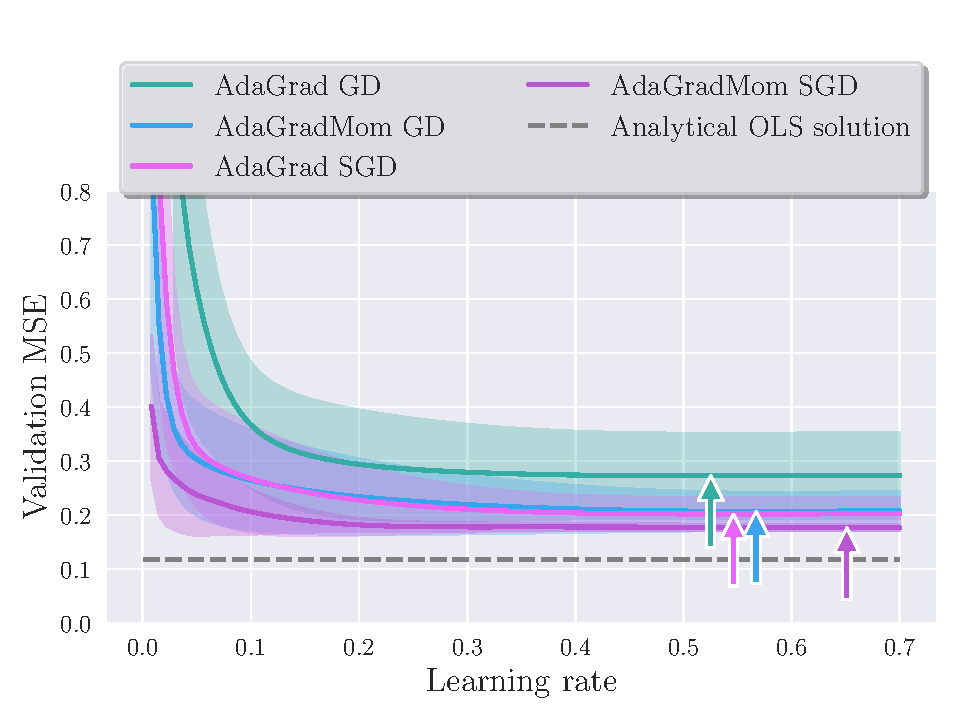
\includegraphics[width=\linewidth]{learning_rates_adagrad}
            \caption{Best MSEs, learning rates: (0.2725, 0.528), (0.2065, 0.570), (0.1810, 0.576), (0.1784, 0.175)}
            \label[fig]{res:fig:lrate3}
        \end{subfigure}
        \hfill
        \begin{subfigure}{.5\textwidth}
            \centering
            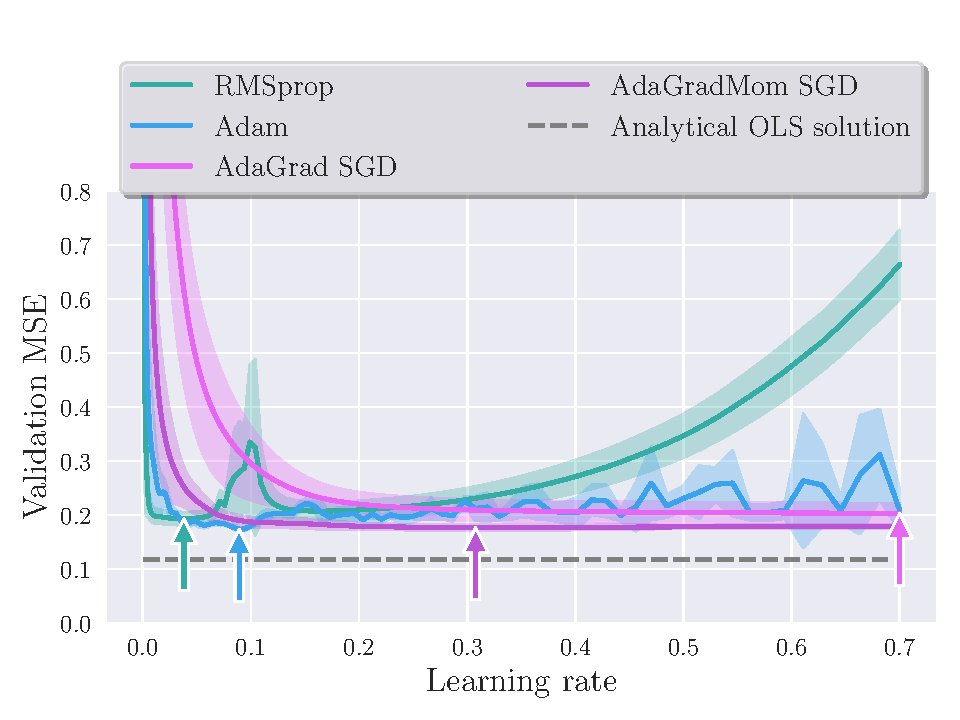
\includegraphics[width=\linewidth]{learning_rates_tunable}
            \caption{Best MSEs, learning rates: (0.1810, 0.576), (0.1784, 0.174), (0.1829, 0.00610), (0.1792, 0.0181)}
            \label[fig]{res:fig:lrate4}
        \end{subfigure}
        \caption{Plots of the validation MSE of the parameters found from optimising the OLS cost function on Franke function data with $n=600$ data points. For the momentum methods we used $\gamma=0.8$. The stochastic methods used 16 batches and 100 epochs, while the standard GD did 100 iterations unless specified otherwise.
        Analytical OLS MSE: 0.1176.}
        \label[fig]{res:fig:lrates}
    \end{figure*}